\documentclass[11pt,letterpaper]{article}
\usepackage[margin=2.5cm,top=3.5cm,bottom=3cm]{geometry}
\usepackage{booktabs}
\usepackage{graphicx}
\usepackage[hidelinks]{hyperref}
\usepackage{microtype}
\usepackage[table,dvipsnames]{xcolor}
\usepackage{longtable}
\usepackage{array}
\usepackage{caption}
\usepackage[T1]{fontenc}
\usepackage{lmodern}
\usepackage{fancyhdr}
\usepackage{amsmath}
\usepackage{titlesec}
\usepackage{enumitem}

\definecolor{wavblue}{RGB}{26,58,92}
\definecolor{wavgray}{RGB}{120,120,120}
\definecolor{wavlight}{RGB}{235,242,250}
\definecolor{wincolor}{RGB}{0,110,0}

\graphicspath{{./}}

\pagestyle{fancy}
\fancyhf{}
\fancyhead[L]{\small\color{wavgray}Manifold-Informed Architecture Benchmark \textemdash\ CIFAR10}
\fancyhead[R]{\small\color{wavgray}\texttt{waverider @ 3c5d283}}
\fancyfoot[C]{\small\color{wavgray}\thepage}
\renewcommand{\headrulewidth}{0.4pt}

\titleformat{\section}{\large\bfseries\color{wavblue}}{}{0em}{}[\color{wavblue}\titlerule]
\titleformat{\subsection}{\normalsize\bfseries\color{wavblue}}{}{0em}{}
\setlength{\parindent}{0pt}
\setlength{\parskip}{4pt plus 1pt}

\begin{document}

\begin{center}
  {\LARGE\bfseries\color{wavblue} Manifold-Informed Architecture Benchmark}\\[6pt]
  {\large CIFAR10: 10 classes, 3,072D input}\\[8pt]
  {\small Generated: 2026-08-04 03:29:24 \quad$|$\quad Apple M5 Max MacBook Pro, 64 GB RAM, 2TB SSD}\\[2pt]
  {\small\texttt{waverider @ 3c5d283} (--abbrev-re
3c5d28344fd5c5ace0b3399593d61b40363afcda) \quad$|$\quad 2026-08-04 03:22:44 +0000}
\end{center}
{\color{wavblue}\noindent\rule{\linewidth}{1.5pt}}
\medskip

\noindent\colorbox{wavlight}{\parbox{\dimexpr\linewidth-2\fboxsep\relax}{
  \smallskip
  \textbf{Best:} Standard (1024$\rightarrow$512)\quad test acc $= 0.5167 \pm 0.0075$\\[2pt]
  \textbf{Manifold:} 3,072D $\rightarrow$ 34D (98.9\%\ noise dimensions)\\[2pt]
  \smallskip
}}
\bigskip

\section{Experimental Setup}

\begin{tabular}{@{}ll@{}}
\toprule
\textbf{Parameter} & \textbf{Value} \\
\midrule
  Dataset & CIFAR10 \\
  Input dimensionality & 3,072D \\
  Classes & 10 \\
  Intrinsic dim ($d$) & 34 \\
  Variance threshold ($\tau$) & 0.9 \\
  Epochs & 60 \\
  Trials & 5 \\
  Batch size & 512 \\
  Learning rate & 0.001 \\
  $k$ neighbors (local PCA) & 50 \\
  Discovery samples & 500 \\
  Samples per class & 10 \\
\bottomrule
\end{tabular}

\section{Manifold Discovery}

Local PCA over the training set, $k = 50$ neighbors. Intrinsic dimensionality $d$ is taken as the maximum per-class maximum at $\tau = 0.9$, clamped to $n_{\mathrm{classes}} = 10$.

\begin{tabular}{@{}rrrrrr@{}}
\toprule
$\tau$ & Mean $d$ & Std & Min & Max & Noise (\%) \\
\midrule
  0.95 & 36.0 & 1.8 & 24 & 40 & 98.8 \\
  0.90 & 28.8 & 1.9 & 18 & 33 & 99.1 \\
  0.85 & 23.6 & 1.9 & 14 & 28 & 99.2 \\
  0.80 & 19.6 & 1.8 & 11 & 24 & 99.4 \\
\bottomrule
\end{tabular}

\subsection{Per-Class Intrinsic Dimensionality}

\begin{tabular}{@{}lrrrr@{}}
\toprule
Class & Mean $d$ & Std & Min & Max \\
\midrule
  frog & 31.6 & 1.8 & 28 & 33 \\
  truck & 31.4 & 1.6 & 28 & 34 \\
  horse & 31.1 & 0.8 & 30 & 33 \\
  automobile & 30.8 & 2.2 & 25 & 33 \\
  deer & 29.2 & 1.5 & 28 & 32 \\
  dog & 28.4 & 0.8 & 27 & 30 \\
  cat & 27.8 & 1.0 & 26 & 29 \\
  bird & 27.7 & 2.1 & 25 & 31 \\
  airplane & 26.5 & 1.2 & 25 & 29 \\
  ship & 25.6 & 1.6 & 22 & 27 \\
\bottomrule
\end{tabular}

\section{Architecture Comparison}

{\small
\begin{tabular}{@{}p{7cm}rccr@{}}
\toprule
\textbf{Architecture} & \textbf{Params} & \textbf{Test Acc ($\mu \pm \sigma$)} & \textbf{Loss} & \textbf{Acc/Kparam} \\
\midrule
  {\color{wincolor}Standard (1024$\rightarrow$512)\,$\star$} & 3,676,682 & $0.5167 \pm 0.0075$ & 4.4642 & 0.0001 \\
  {Wide Manifold (d+1, d=34)} & 107,915 & $0.4558 \pm 0.0038$ & 1.6858 & 0.0042 \\
  {Manifold (d=34)} & 104,832 & $0.4585 \pm 0.0026$ & 1.6821 & 0.0044 \\
  {Manifold + ManifoldAdam (d=34)} & 104,832 & $0.4731 \pm 0.0035$ & 1.4881 & 0.0045 \\
  {ManifoldAdam (1024$\rightarrow$512, proj$\rightarrow$34D)} & 3,676,682 & $0.4623 \pm 0.0094$ & 3.3072 & 0.0001 \\
  {PCA$\rightarrow$34D + MLP (2d$\rightarrow$d)} & 5,076 & $0.4912 \pm 0.0046$ & 1.4503 & 0.0968 \\
  {Intrinsic Dim (PCA$\rightarrow$34D$\rightarrow$output)} & 1,540 & $0.4675 \pm 0.0051$ & 1.4954 & 0.3036 \\
\bottomrule
\end{tabular}
}

\smallskip
{\small $\star$ = best performing architecture}

\section{Key Findings}

\begin{itemize}[leftmargin=*,itemsep=3pt]
  \item \textbf{Best architecture:} Standard (1024$\rightarrow$512) \textemdash\ test accuracy $0.5167 \pm 0.0075$
  \item \textbf{Manifold compression:} 3,072D $\rightarrow$ 34D (98.9\%\ of ambient dimensions carry no structure)
\end{itemize}

\clearpage
\section{Result Figure}

\begin{figure}[htbp]
\centering
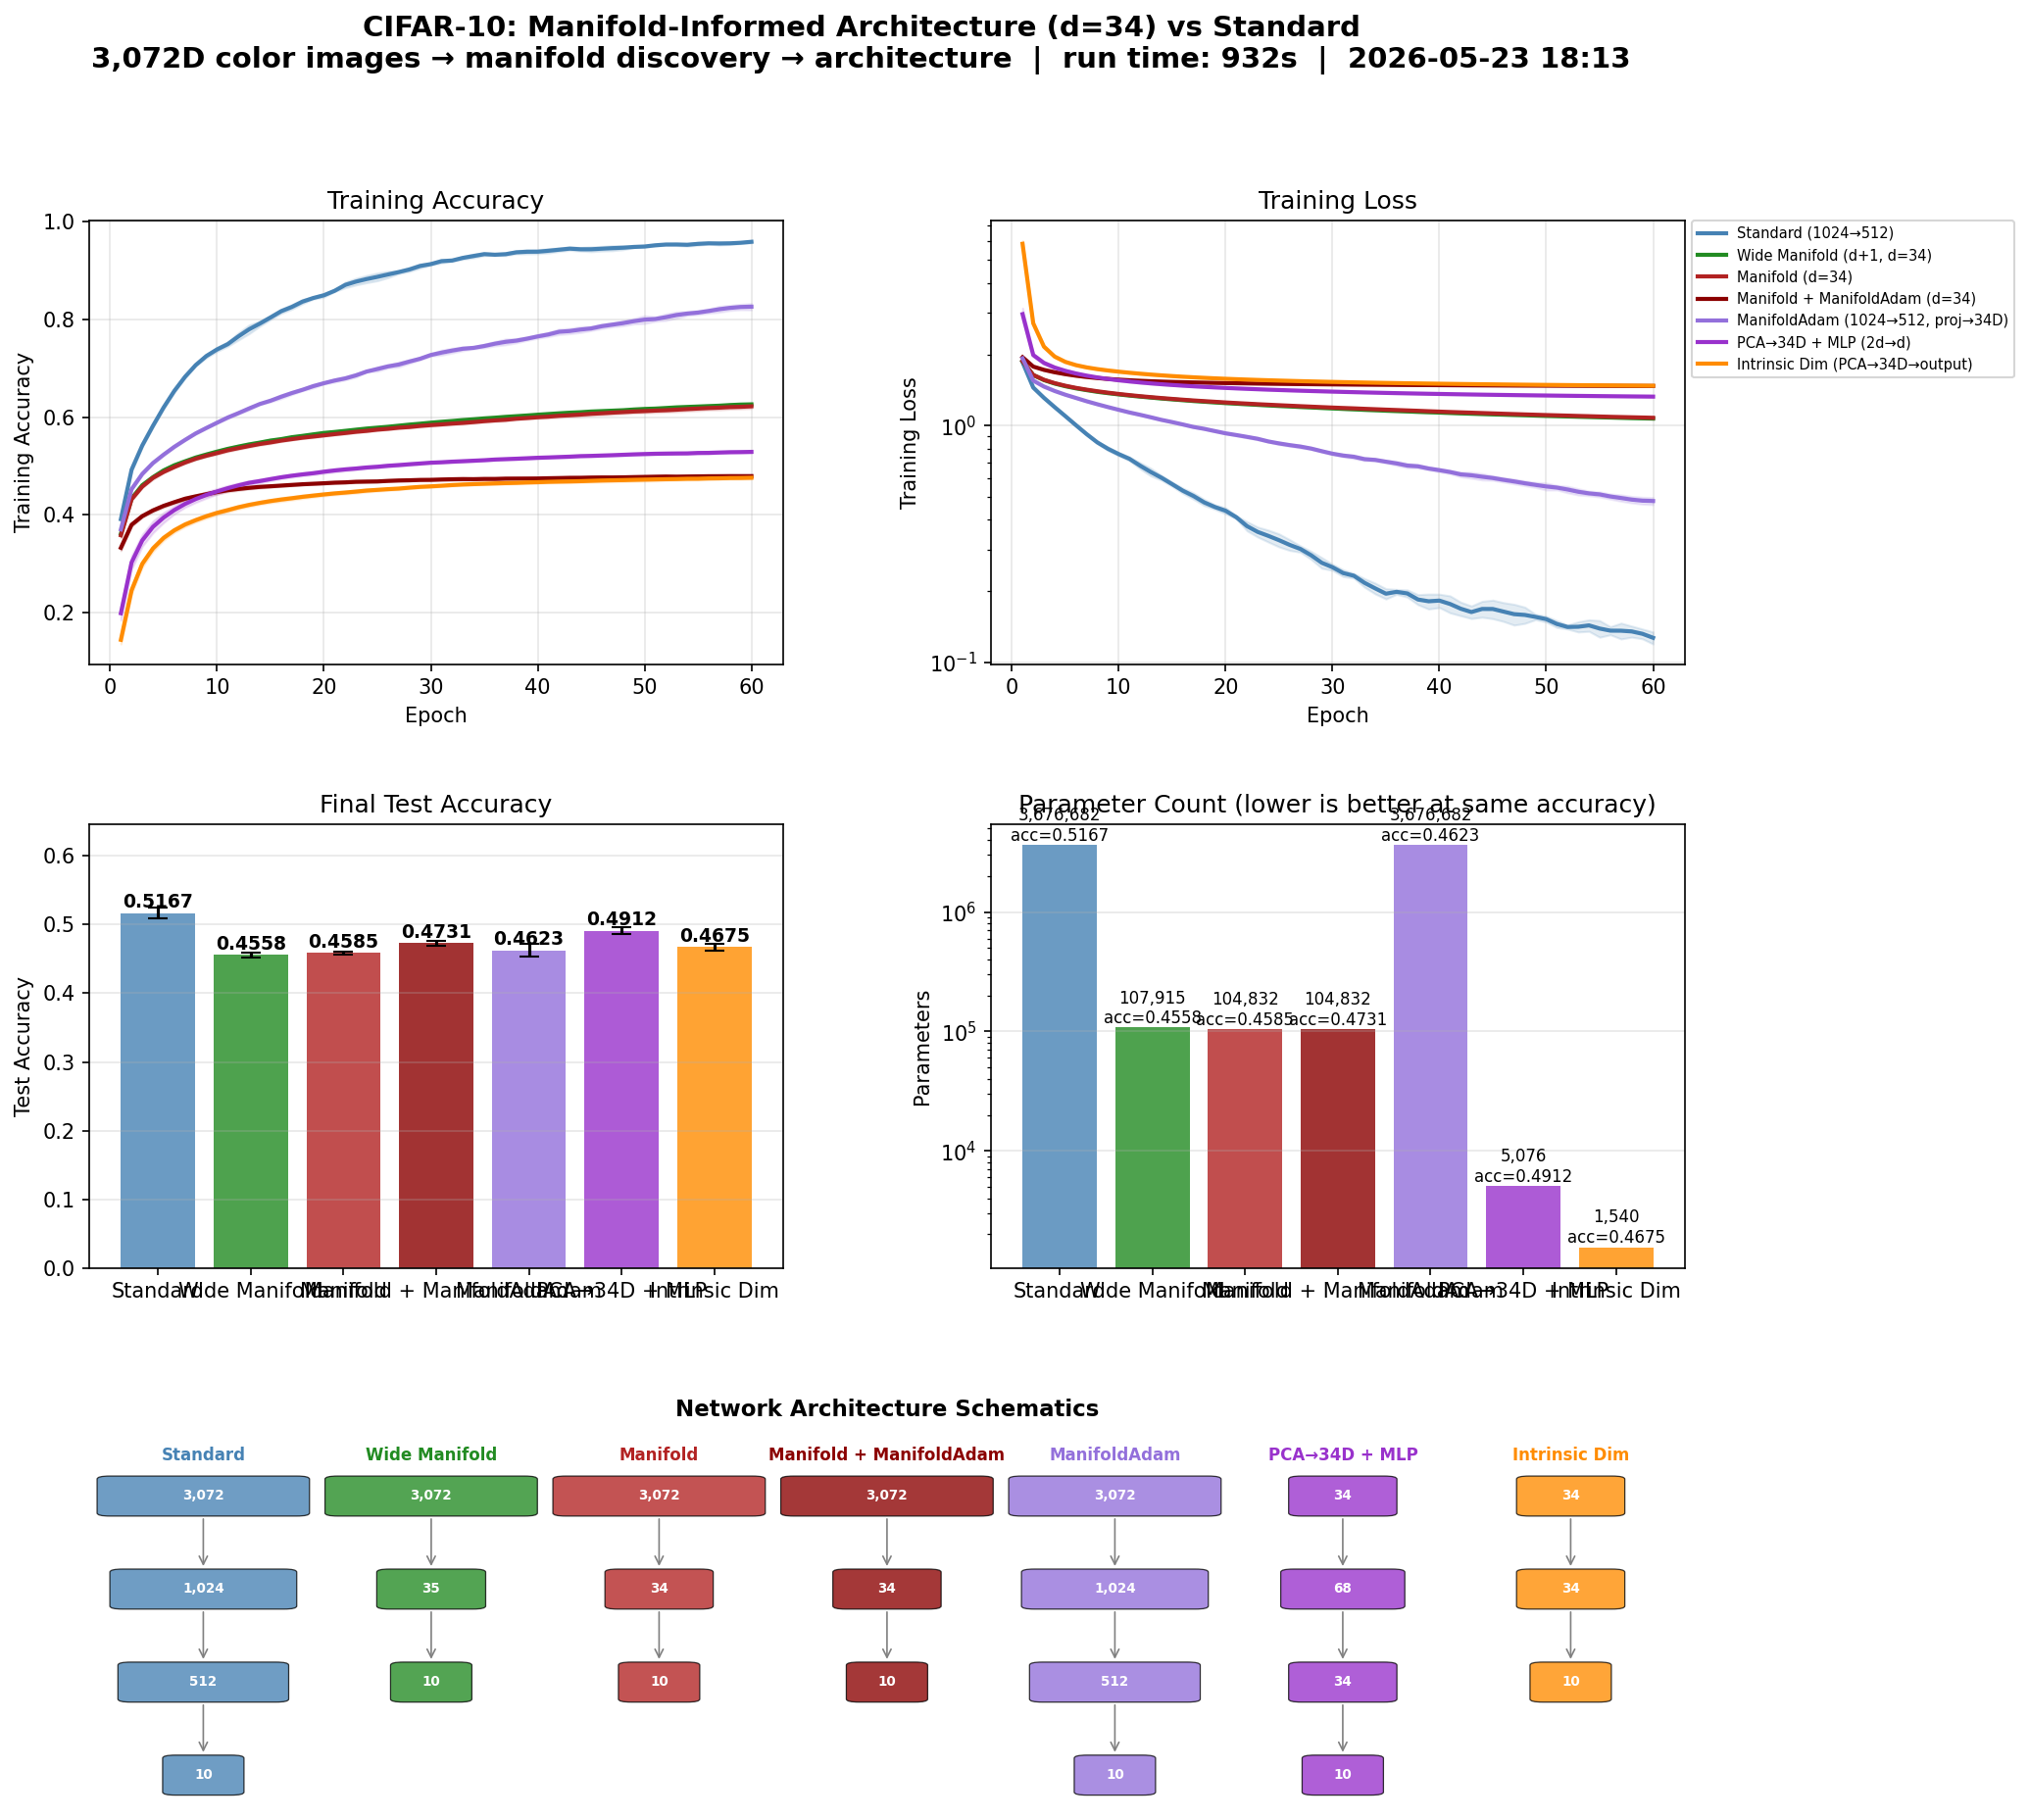
\includegraphics[width=\textwidth]{cifar10_architecture_results}
\caption{CIFAR10 manifold-informed vs.\ standard architecture comparison. $d = 34$, 60 epochs, 5 trials.}
\end{figure}

\section{Provenance}

\begin{tabular}{@{}ll@{}}
\toprule
\textbf{Item} & \textbf{Value} \\
\midrule
  Repository & \href{https://github.com/Flux-Frontiers/waverider}{Flux-Frontiers/waverider} \\
  Commit & \texttt{3c5d283} (--abbrev-re
3c5d28344fd5c5ace0b3399593d61b40363afcda) \\
  Commit date & 2026-08-04 03:22:44 +0000 \\
  Commit message & docs(readme): add holographic-rendering Breaking News section; audit fixes \\
  Python & 3.12.3 \\
  TensorFlow & 2.21.0 \\
  Device & CPU (forced) \\
  Host & vm \\
  OS & Linux-6.18.5-fc-v18-x86\_64-with-glibc2.39 \\
  Machine & Apple M5 Max MacBook Pro, 64 GB RAM, 2TB SSD \\
  Generated & 2026-08-04 03:29:24 \\
\bottomrule
\end{tabular}

\end{document}
